The construction of a valid barrier certificate can be a non-trivial task, as it was seen in the construction of a \gls{cbf} for the second order system in \autoref{subsec:cbf-2order}. And with increasing order of the system for which safety need to be guaranteed the difficulty rapidly increases. Hence it is desired to use a more methodical approach to construct barrier certificates, and for this purpose the MATLAB toolbox SOSTOOLS can be used \citep{bib:prajna_framework} (for acquisition, see \autoref{app:sostools}). This toolbox requires that the problem is cast as a \gls{sos} program, which is why this chapter is dedicated to give an introduction to the concept of \gls{sos} and how the barrier certificate definition can be recast as an \gls{sos} problem.

%This chapter describes and establishes the theory applied when the analysis approach is adopted, i.e. to analyse if a given closed loop system is safe.
Now, instead of manually constructing a \gls{cbf} for the open-loop system in order to design a safety controller from it, a barrier certificate for a closed-loop system is sought with SOSTOOLS.
When a barrier certificate can be found for a closed-loop system $f_{cl}(x)$ according to \autoref{def:barrier_certificate} this signifies a verification that the system, and hence the controller, is safe according to the outlined problem. 
%Barrier certificates can be used to (in)validate the safety compliance of a controller design by testing if a barrier certificate can be found according to \autoref{eq:barrier_constraints} for the closed-loop system $f_{cl}(x)$. 
SOSTOOLS can be used to search for a polynomial barrier certificate given that: \citep{bib:prajna_framework}
\vspace{-2mm}
\begin{itemize}
	\itemsep-0.5mm
\item The vector field of the closed-loop system is polynomial.
\item The sets $\mathcal{X}$, $\mathcal{X}_0$ and $\mathcal{X}_u$ can be described as intervals in each of the $n$ dimensions, which can be defined through positivity of polynomials on each interval.
\end{itemize}
%are described by polynomial (in)equalities, a polynomial barrier certificate can be constructed using \gls{sos} optimization. 

\vspace{-1mm}
Furthermore the recasting of the barrier certificate definition as an \gls{sos} problem requires the use of \gls{sos} polynomials. An \gls{sos} polynomial $p(\mathbf{x})$ is denoted by $p\in$ \gls{SigmaSOS} signifying that $p$ is a polynomial in the variable $\mathbf{x}$ with coefficients in the set of \gls{sos} variables: $\Sigma$. A polynomial $p(\mathbf{x})$ is \gls{sos} if there exist polynomials $f_1,\dots,f_m$ such that \citep{bib:parrilo_sdp}
\vspace{-2mm}
\begin{equation}
p(\mathbf{x}) = \sum_{j=1}^{m}f_j^2(\mathbf{x}) \label{eq:sos_f_squared}
\end{equation}
%
%A \gls{sos} program is a convex optimization problem of the form \citep{bib:prajna_framework,bib:sostools}
%\begin{subequations}
%\begin{align}
%&\min_{c}\, w^Tc\\
%&\text{subject to} \qquad
%q_{i,0}(x) + \sum_{j=1}^{m} q_{i,j}(x)g_j(x) \,\,\,\in \Sigma[x]
%\qquad \text{for}\quad
%i=1,\dots, p
%\end{align}
%\end{subequations}
%\vspace*{-4mm}
%\begin{tabular}{rl}
%where &\\
%$w$ & is a vector of weighting coefficients of the linear objective function\\
%$c$ & is a vector formed by the (unknown) scalar real coefficients of $g_j(x)$\\
%$g_j(x)$ & are polynomials in $x$\\
%$q_{i,j}(x)$ & are given \gls{sos} polynomials with fixed coefficients\\
%$\Sigma$ & denotes the set of \gls{sos} variables\\
%\subsection*{Notation}

\vspace{-2mm}
A short illustrating example is given initially with the intention to provide some understanding about \gls{sos} polynomials and the notation applied.
\vspace{-0.0cm}
\begin{exa}[Sum of Squares Polynomial]
Consider the second order polynomial $f_1(x)=a\,x^2 + b\, x + c$. Comparing to the structure of an \gls{sos} polynomial  $f_2(x) = (d + e\,x)^2= d^2 + 2de\,x + e^2 x^2$, it is seen that if the relationship:
\begin{flalign*}
a = e^2, \mm  \mm b =  2de, \mm \mm  c = d^2 \kk \Big( \text{or simply $b=2\sqrt{ac}$} \Big)
\end{flalign*} 
holds, then $a,b,c$ are \gls{sos} variables, denoted by $a,b,c \in \Sigma$, because they are the coefficients in an \gls{sos} polynomial. %In that sense, $\Sigma$ denotes the set of \gls{sos} variables. 
It can additionally be stated that:
\begin{flalign*}
f_1(x) \in \Sigma[x]
\end{flalign*}
where $\Sigma[x]$ denotes a set of polynomials in $x$ with coefficients in $\Sigma$, i.e. $f_1(x)$ is \gls{sos}.
\end{exa}

Declaring a polynomial in SOSTOOLS is done by defining a monomial vector for which the program solves for polynomial coefficients.
Introducing the notion of a monomial vector as a vector \gls{monomialvec} in $\mathbf{x}$ of degree $deg$; e.g. if $\mathbf{x}\in\mathbb{R}^2$ and $deg=[0:2]$ each entry has the form $x_1^ax_2^b$ with exponents $a+b=deg=0,...,2$ i.e.
\vspace{-3mm}
\begin{equation}
\mathbf{z}=[x_1^0x_2^0\quad x_1^1x_2^0\quad x_1^0x_2^1\quad x_1^2x_2^0\quad x_1^1x_2^1\quad x_1^0x_2^2]^T=[1\quad x_1\quad x_2\quad x_1^2\quad x_1x_2\quad  x_2^2]^T
\label{eq:monomial_example}
\end{equation} 

\vspace{-1mm}
Now, according to \citep{bib:parrilo_sdp} an \gls{sos} polynomial $p\in \Sigma[\mathbf{x}]$ can be formulated on a quadratic form comprising a coefficient matrix and a monomial vector
\vspace{-1mm}
\begin{equation}
p = \mathbf{z}^T \mathbf{Q} \, \mathbf{z}, \qquad\qquad p\geq 0 \quad \forall \,\, \mathbf{x}\in\mathbb{R}^n %\setminus \{0\}
\label{eq:sos_polynomial}
\end{equation}
\begin{tabular}{rl}
where &\\
$\mathbf{z}$ & is a monomial vector in $\mathbf{x}\in \mathbb{R}^n$\\
\gls{Q} & is a real positive semidefinite symmetric coefficient matrix\\
\end{tabular}\\

With monomials and \gls{sos} polynomials defined, a polynomial barrier certificate can now be constructed. An \gls{sos} description of a problem, however, is a global description of nonnegativity (positive or zero), and it is desired to set up local requirements for the barrier polynomial on each of the sets $\mathcal{X}$, $\mathcal{X}_0$ and $\mathcal{X}_u$. % as given by \autoref{def:barrier_certificate}.

A way to be able to define nonnegativity locally is to use Positivstellens\"atze.
A Positivstellensatz is a structure theorem of a  polynomial which is positive on some set, and gives an algebraic certificate that a solution exists for a system of real polynomial inequalities \citep{bib:positivstellensatz}. 
%Obtain certificates of positivity on a basic semialgebraic set $\mathbb{K}\subseteq\mathbb{R}^n$. \citep{bib:sos_putinar_laurent}
%A Positivstellensatz defines the regions of a semialgebraic set where a function is positive. 
%non-commutative Positivstellens\"{a}tze characterize things like a polynomial $p$ being positive where another polynomial $q$ is positive
In Putinar's Positivstellensatz, presented in \autoref{def:putinar}, a compact set $\mathbb{K}\subset\mathbb{R}^n$ (a strict subset of the state-space, i.e. not including the entire state-space) is defined by the nonnegativity of some polynomials $g_j$.
Now the positivity of a polynomial $h$ on the set $\mathbb{K}$ can be expressed in terms of a weighted sum of these polynomials $g_j$ with \gls{sos} polynomials as coefficients $q_j\in\Sigma[\mathbf{x}]$ \citep[pp 184-186]{bib:sos_putinar_laurent},\citep[pp 28-29]{bib:sos_putinar_lasserre}.\\

 
\vspace{-2mm}
\begin{thm}[Putinar's Positivstellensatz]\label{def:putinar}
Given the finite family of polynomials $(g_j)_{j=1}^m$ and the subset $Q(g)$ %is called the quadratic module 
generated by the family $(g_j)_{j=1}^m$ \citep[p 29]{bib:sos_putinar_lasserre}
\begin{subequations}\label{eq:putinar}
\begin{align}
\text{polynomials} \qquad & (g_j)_{j=1}^m \in\mathbb{R}[\mathbf{x}]\label{eq:polynomials_g}\\
\text{set} \qquad & Q(g)=Q(g_1,...,g_m)\equiv\left\{\left.q_0+\sum\limits_{j=1}^{m}q_jg_j\,\,\right| \, (q_j)_{j=0}^m\in\Sigma[x]\right\}\label{eq:putinar_set_sos}
\end{align}
\end{subequations}
Assume that there exists a function $u(\mathbf{x})\in Q(g)$ such that the level set $\{\mathbf{x}\in\mathbb{R}^n \,\,|\,\, u(x)\geq 0\}$ is compact \citep[p 29]{bib:sos_putinar_lasserre}.
Given a polynomial $h$ and the compact basic semialgebraic set $\mathbb{K}$  defined by the nonnegativity of the polynomials $g_1,\dots, g_m$  
\begin{subequations}
\begin{align}
\text{polynomial} \qquad & h \in\mathbb{R}[\mathbf{x}]\\
\text{set} \qquad & \mathbb{K}\equiv\left\{\left.\mathbf{x}\in \mathbb{R}^n\,\, \right| \, (g_j)_{j=1}^m\geq0\right\}\qquad\qquad\qquad\qquad\qquad\quad\label{eq:setK}
\end{align}
\end{subequations}
If the polynomial $h$ is strictly positive on the set $\mathbb{K}$, then $h\in Q(g)$, which means that $h$  can be formulated as
\begin{equation}\label{eq:sos_barrier}
h = q_0+\sum\limits_{j=1}^{m}q_jg_j
\end{equation}
\end{thm}

\vspace{-16mm}
%\section{Using Sums of Squares to Construct a Barrier Certificate}
%\vspace*{-7mm}
\begin{figure}[H]
\centering
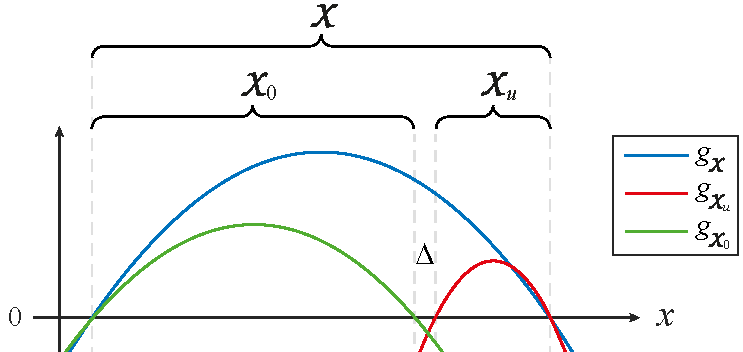
\includegraphics[width=0.6\textwidth]{1stordersys_staticlimits_g.pdf}
\caption{Example of $g$-polynomials defining each of the sets $\mathcal{X}$, $\mathcal{X}_u$ and $\mathcal{X}_0$ by their nonnegativity, with a distance $\Delta$ between the safe and unsafe sets.}
\label{fig:1stordersys_staticlimits_g}
\end{figure}

In \autoref{eq:setK} the region of nonnegativity of the polynomial(s) $(g_j)_{j=1}^m$ define the extent of the set $\mathbb{K}$, the $g$s being  polynomials in the state variables $x$ as defined by \autoref{eq:polynomials_g}, e.g. in 1D Cartesian space $g(\mathbf{x})$ may be a parabola which is positive-valued on the interval $\mathbf{x}\in[a,b]$, hence defining the semialgebraic set $\mathbb{K}=\{\mathbf{x}\in[a,b]\}$. In this way appropriate polynomials $g_j$ can be constructed  to define each of the sets $\mathcal{X}$, $\mathcal{X}_0$ and $\mathcal{X}_u$ as given by \autoref{def:barrier_certificate}. An example of a polynomial $g_1$ for each of the sets is sketched in \autoref{fig:1stordersys_staticlimits_g}.

The variables $(q_j)_{j=1}^m$ in \autoref{eq:putinar_set_sos} are \gls{sos} and thereby nonnegative per definition. Hence from the definition of the $g$s and $q$s it can be seen from \autoref{eq:sos_barrier} that the polynomial $h$ is positive on the set $\mathbb{K}$.
% as defined by  being positive  in the region $\mathbb{K}$.
Outside the set $\mathbb{K}$ one or more $g_j$s are negative, and hence the sign of $h$ cannot be determined outside $\mathbb{K}$.
Rearranging \autoref{eq:sos_barrier} to
\vspace{-2mm}
\begin{equation}
\underbrace{q_0(\mathbf{x})}_{\geq 0\,\,\forall \,\,\mathbf{x}} = h(\mathbf{x}) - \sum _{j=1}^{m}\,\,\,\underbrace{q_j(\mathbf{x})}_{\geq 0\,\,\forall \,\,\mathbf{x}}\,\,\,\underbrace{g_j(\mathbf{x})}_{\geq 0 \,\,\forall \,\,\mathbf{x}\in\mathbb{K}} \kk \in\Sigma[\mathbf{x}]\label{eq:putinar_sos}
\end{equation} 

\vspace{-1mm}
however, the right-hand expression will always be nonnegative due to the SOS equality. Using SOSTOOLS  it is possible to solve for the unknown $h$ setting up a number of \gls{sos} inequalities corresponding to defining the right-hand side of \autoref{eq:putinar_sos} as being nonnegative. %:  $expr\in\Sigma[x]$ (corresponding to $expr\geq 0$) on each set $\mathbb{K}$. 

\section{Recasting the Barrier Certificate Definition}
\vspace{-2mm}
Now \autoref{eq:putinar_sos} can be seen as a template for the reformulation of the requirements for a barrier certificate in \autoref{def:barrier_certificate}.
Setting up each of the requirements for the barrier certificate $B(\mathbf{x})$ on each of the  semialgebraic sets $\mathcal{X}$, $\mathcal{X}_u$ and $\mathcal{X}_0$, is a matter of defining one or more polynomials $g_j(\mathbf{x})$ for each set such that the intersection of the nonnegative regions of the polynomials outline the set.
E.g. in order to define the region $\mathcal{X}_u\subset\mathcal{X}\subset\mathbb{R}$ construct a polynomial $g(\mathbf{x})$ such that it is positive within the unsafe interval and its zero level set constitutes the desired border of the region. An example of a polynomial $g(\mathbf{x})$ defining the region $\mathcal{X}_u$ is seen in \autoref{fig:1stordersys_staticlimits_g} as the red curve. If several polynomials $g_j(\mathbf{x})$ are used to define $\mathcal{X}_u$, the set is defined by the nonnegative intersection region, i.e. the subset of the state-space where all of the $g_j(\mathbf{x})$s are nonnegative.

When the polynomials $g_j(\mathbf{x})$ have been defined for each of the sets, the polynomial $h(\mathbf{x})$ in \autoref{eq:putinar_sos} is substituted according to \autoref{def:barrier_certificate}, such that $h(\mathbf{x})\geq 0$ on the relevant set. That is, when defining $\mathcal{X}$ according to \autoref{cer3}, the polynomial $h(\mathbf{x})$ can be written as $-L_{f_{cl}}B(\mathbf{x})$ and when defining $\mathcal{X}_0$ use $h(\mathbf{x})=-B(\mathbf{x})$ according to \autoref{cer1}. However, when defining $\mathcal{X}_u$ according to \autoref{cer2}, the positivity constraint on $B(\mathbf{x})$ has to be transformed into a nonnegativity constraint. This can be done by introducing a small scalar value $\bar{\epsilon}>0$, such that $B(\mathbf{x})\geq \bar{\epsilon} $ or identically $B(\mathbf{x})-\bar{\epsilon}\geq 0$ which can now be substituted for $h(\mathbf{x})$.

\begin{defn}[Barrier Certificate Recast to \gls{sos} Formulation]\label{def:barrier_sos}
In summary, referring to the requirements for a barrier certificate in \autoref{def:barrier_certificate} and the \gls{sos} formulation of the polynomial $h$ in \autoref{eq:putinar_sos} based on Putinar's Positivstellensatz, the inequalities defining the barrier certificate $B(\mathbf{x})$ can be set up as
\vspace{-2mm}
\begin{subequations}\label{eq:barrier_constraints_putinar}
\begin{flalign}
&&	-B(\mathbf{x}) &\geq 0 \kk  \forall \hspace{2mm} \mathbf{x} \in \mathcal{X}_0 \qquad\quad \Leftarrow& 	-B(\mathbf{x}) - \sum _{j=1}^{m}q_jg_j &\,\,\,\in \Sigma[\mathbf{x}] &&& \label{cer1_putinar}\\
&&	B(\mathbf{x})-\bar{\epsilon} &\geq 0 \kk  \forall \hspace{2mm} \mathbf{x} \in \mathcal{X}_u \qquad\quad \Leftarrow& 	B(\mathbf{x})-\bar{\epsilon} - \sum _{j=1}^{m}q_jg_j &\,\,\,\in \Sigma[\mathbf{x}] &&&\label{cer2_putinar} \\
&&	-L_{f_{cl}}B(\mathbf{x}) &\geq 0 \kk  \forall \hspace{2mm} \mathbf{x} \in \mathcal{X} \qquad\quad\,\, \Leftarrow& 	-L_{f_{cl}}B(\mathbf{x}) - \sum _{j=1}^{m}q_jg_j &\,\,\,\in \Sigma[\mathbf{x}] &&& \label{cer3_putinar}
\end{flalign}
\end{subequations}
\end{defn}
%Note that the inequality is on positivity in \autoref{cer2} whereas it is on nonnegativity (being \gls{sos}) in \autoref{eq:putinar_set_sos}. By introducing an arbitrarily small $\epsilon>0$ the positivity constraint can be cast as the nonnegativity constraint in the  SOS inequality of \autoref{cer2_putinar}. %This is, however, not considered an issue in the scope of this project, as the position accuracy of the robot is not on the submillimeter level. 

%\vspace{-15mm}
With this formulation the Lie derivative is required to be nonpositive on set $\mathcal{X}$ and the barrier certificate is required to be nonpositive on the safe set $\mathcal{X}_0$ and greater than or equal to the constant \gls{epsilonbar} on the unsafe set $\mathcal{X}_u$. When defining the sets, the safe and unsafe regions must be separated by some distance \gls{Delta}. This is illustrated in \autoref{fig:sos_delta1}.

The task of searching for a barrier certificate validating system safety is now a matter of the fairly easy construction of the polynomials $g_j(\mathbf{x})$ to define the desired outline of each of the sets $\mathcal{X}$, $\mathcal{X}_u$ and $\mathcal{X}_0$, as in the example in \autoref{fig:1stordersys_staticlimits_g}, in SOSTOOLS. However, it is also a matter of deciding the polynomial degree (through monomials) of $B(\mathbf{x})$ and of each of the \gls{sos} polynomials $q_j(\mathbf{x})$. As small a degree "as possible" is desired for all monomials, but it may be necessary to increase the degree iteratively. This introduces numerical errors, which may require that the size of $\bar{\epsilon}$ must be increased. When no solution can be found, it may be necessary to increase the  distance $\Delta$ separating the safe and unsafe regions, i.e. contract the safe region by altering the polynomials $g_j(\mathbf{x})$ outlining the region.

%\textcolor{red}{Bemærk, at denne sætning ikke siger hvor høj grad I skal vælge qerne. (husk at tænke på dette)}

\begin{figure}[H]
\centering\hspace{10mm}
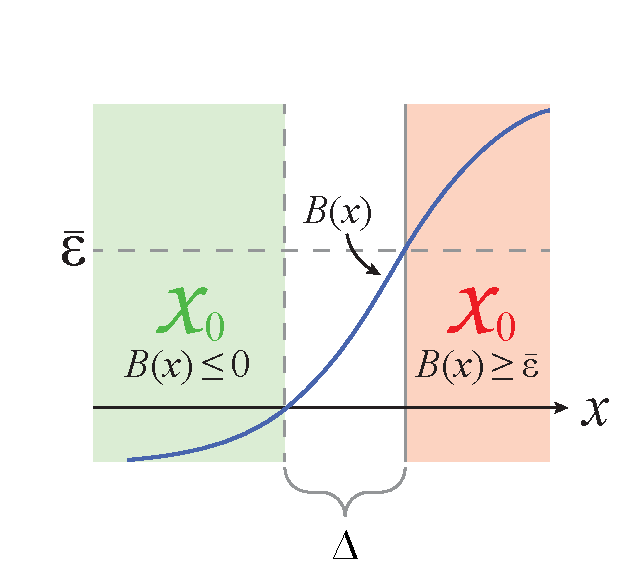
\includegraphics[width=0.3\textwidth]{sos_delta.pdf}
\caption{The value of $B(x)$ on the unsafe set is at least the small positive value $\bar{\epsilon}$, while the value on the safe set is nonpositive. This requires that the two sets are separated by a small distance\,$\Delta$.}
	\label{fig:sos_delta1}
\end{figure}

In the following chapter the syntax for SOSTOOLS is introduced and barrier certificates are sought to validate safety of systems, based on linear closed-loop systems representing the da Vinci robot from the preceding chapters.

 
	


%\section{Approach for Verification of System Safety}
%
%The following chapters present the safety verification of first- and second order systems in 1D and 3D with static and dynamic boundaries using Putinar's Positvstellensatz in the SOSTOOLS framework. The same systems are used for the analysis as in \autoref{part:cbf}, and to the extent it is possible, also the same (pole placement design) controllers are tested. \textcolor{red}{Correct this when the chapters are written!!!}

